\chapter{Plano de Gestão de dados}
\label{plano_de_gestao_de_dados}
\section{Descrição da forma como os dados são recolhidos, armazenados e manipulados}
Os dados inseridos no sistema ePadaria são recolhidos através do sistema com ligação á base de dados e diretamente lá armazenados. Apenas alguns dados podem ser manipulados, parte do cliente poderá mudar os seus dados pessoais que também mudam diretamente na altura na própria base de dados, mas após efetuado e pago um pedido o cliente não poderá fazer alterações aos produtos pedidos, o funcionário pode adicionar, remover ou alterar produtos pelo ePadaria e terá acesso aos pedidos feitos dos clientes ,em que pode dar como concluído e esse pedido passa para a tabela dos pedidos concluídos dentro da base de dados e que o funcionário também poderá ter acesso. Quanto aos dados pessoais do funcionário só terá acesso ao username e password e caso houvesse necessidade de alterar a padaria teria de contactar o ePadaria para o fazer diretamente na base de dados.
\section{Apresentação da base de dados}

Na imagem abaixo encontra-se estruturado as tabelas da base de dados do ePadaria,é uma base de dados simples sem a necessidade de chaves externas,visto que um funcionário pode inserir pedidos nas base de dados sem o cliente estar registado no ePadaria e o cliente pedir um produto com alguma alteração do original.
\begin{figure}[H]
	\centering
	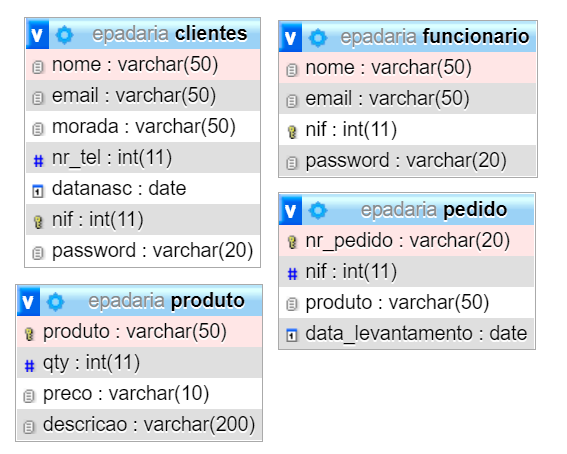
\includegraphics{bd}
	\caption{Estrutura da base de dados do ePadaria}
	\label{fig:bd}
\end{figure}

\section{Permissões de acesso a dados}
A base de dados do ePadaria só pode ser diretamente acedida pelos gestores do projeto tendo em conta a conformidade com o RGPD na proteção e tratamento de dados.\\
Apenas os utilizadores/clientes poderão aceder aos respetivos dados através da sua conta, o funcionário apenas pode visualizar os dados do cliente encontrados no pedido, os restantes dados como password e e-mail apenas os gestores e o próprio utilizador/cliente é que terá acesso.\\
No caso de haver algum problema ou perda com os dados de acesso de um funcionário a única maneira de recuperar esses dados ou alterá-los é pelos gestores/apoio técnico do sistema, já que ao contrário dos utilizadores não podem criar conta, mas ao adquirir o ePadaria é criado os dados para o respetivo log in de cada funcionário. Apesar de um funcionário perder os seus dados de acesso á que ter em atenção que este não tem acesso aos dados dos colegas de trabalho nem deve, cada funcionário como tem o seu respetivo log in caso algo ocorra dentro da padaria de conflitos ou erros é possível ver como é apresentado o nome do funcionário, mas se ocorrer partilha de dados entre funcionários dentro do estabelecimento e usem os acessos uns dos outros o ePadaria não se responsabiliza, o que poderá fazer é dar uma nova password a cada funcionário.

\section{Conformidade com o RGPD (GDPR)}
O ePadaria tem conformidade com o RGPD, com o objetivo de proteger a privacidade dos dados pessoais, enfrentando vários desafios para uma conformidade de cumprimento com o RGPD.\\
O RGPD segue um conjunto de artigos que ajudam a manter esses dados seguros, desde alguns:\\
-\textbf{Tratamento}: Uma ou mais operações efetuadas sobre os dados pessoais por meios automatizados ou não automatizados, como a recolha, o registo, a organização, a estruturação, a
conservação, a adaptação ou alteração, a recuperação, a consulta, a utilização,
a divulgação por transmissão, difusão ou qualquer outra forma de
disponibilização, a comparação ou interconexão, a limitação, o apagamento
ou a destruição (Artº 4º,nº 2);\\
-\textbf{Limitação do tratamento} (Artº4º, nº3);\\
-\textbf{Definição de perfis}: Qualquer forma de tratamento automatizado de dados pessoais que consista
em utilizar esses dados pessoais para avaliar certos aspetos pessoais de uma
pessoa singular, nomeadamente para analisar ou prever aspetos relacionados
com o seu desempenho profissional, a sua situação económica, saúde,
preferências pessoais, interesses, fiabilidade, comportamento, localização ou
deslocações.(Artº 4º, nº 4); \\
-\textbf{Pseudonomização} (Artº 4º, nº 5);\\
-\textbf{Responsável pelo tratamento}: A pessoa singular ou coletiva, a autoridade pública, a agência ou outro organismo que, individualmente ou em conjunto com outras, determina as finalidades e os meios de tratamento de dados pessoais (Artº 4º, nº 7); \\
-\textbf{Consentimento} (Artº 4º, nº 11);\\
-\textbf{Princípio da minimização dos dados}: Os dados pessoais são adequados, pertinentes e limitados ao que é necessário relativamente às finalidades para as quais são tratados (Artº 5º, nº 1 c));\\
-\textbf{Princípio da integridade e confidencialidade} (Artº 5º, nº 1 f));\\

\section{Estado inicial da base de dados}
A base de dados do ePadaria contem alguns exemplos de produtos listados quando é entregue a um cliente,assim este terá perspetiva de como fica os produtos listados no sistema.O cliente que receber pode eliminar esses exemplos ou pedir ao encarregados pela ePadaria para o fazer.
\section{Tarefas de carregamento/povoamento inicial de configurações de dados}
Ao fornecer o ePadaria á padaria que adquiriu o sistema, já se encontra alguns dados de exemplo inseridos, aos quais principalmente produtos e pedidos, quem tem a responsabilidade de inserir esses dados e fazer a sua configuração é algum dos gestores do ePadaria, em que os respetivos funcionários da padaria poderão eliminá-los quando quiserem. \\
Caso haja a necessidade de fazer alguma alteração ou configuração em um pedido ou produto que o funcionário ou cliente não esteja a conseguir, o funcionário tem o dever de contactar o suporte técnico a pedir ajuda e essa pessoa irá ajudar alterando diretamente na base de dados.

